In this section, we (1) introduce the \zop\ approach, (2) describe how we can create a model that encodes training waveform features and (3) use this model to predict the path taken during an unknown execution using only the waveform produced by this execution without using \textit{any} runtime instrumentation.


The goal of \zop\ is to compute code profiling information without any instrumentation. Figure~\ref{fig:overviewzosp} shows a high-level overview of our approach. As the figure shows, \zop\ has two main phases. In the \textit{training phase}, \zop\ runs instrumented and uninstrumented versions of the program against a set of training inputs, records EM emanations for these executions, and builds a model that associates the recorded waveforms with the code subpaths that generated them.  In the \textit{profiling phase}, \zop\ records the EM waveform generated by an execution of a vanilla (\ie completely uninstrumented) version of the program, finds the closest match between sections of this waveform and the waveforms in the training model, and uses the matching subpaths to predict the overall path taken by the execution being profiled. \zop\ implements these two high-level phases in the steps and substeps shown in the workflow portrayed in Figure~\ref{fig:system_diagram}. In the next sections, we explain the different steps and substeps in this workflow in detail.

\subsection{Training 1}
\label{sec:training-1}

The left part of Figure~\ref{fig:system_diagram} shows the Training~1 phase of the \zop\ approach.  During Training~1, \zop\ runs an instrumented version of the system against a set of training inputs.  This step is needed to reconstruct a graph model of the program's states, to determine the timing of each subpath, and to establish the correspondence between subpaths and the EM waveforms they generate.  We refer to the instrumentation points as \hbox{``markers''} since they are used to ``mark'' the time of each executed instrumentation point in the EM waveform. In order to ensure optimal placement of these markers for generating accurate profiling information, the level of granularity of the inserted instrumentation points (markers) is critical.

\begin{figure}[tb]
\includegraphics[width=5in]{../issta_profile/profiling/figures/overviewzosp}
% \vspace{-8pt}
\caption{High-level view of our approach.}
\label{fig:overviewzosp}
\end{figure}

\begin{figure*}[tb]
\includegraphics[width=\textwidth]{../issta_profile/profiling/figures/workflowzosp}
\caption{Workflow of \zop. (Note that we repeat some elements to reduce clutter, improve clarity, and better separate the different  steps of the approach; that is, multiple elements with the same namerepresent the same entity.)}
\label{fig:system_diagram}
\end{figure*}

% SPACE \subsubsection{Operating at the Right Level of Granularity}
%9)Reviewer1:In 3.3.1, ``statements'' should be ``instructions''/''basic blocks''.
In general, matching the EM emanations waveform from an unknown execution path to example waveforms for known execution paths is not a simple task. Matching complete program executions is clearly not an option, as it would require observing all possible executions to build a model. An ideal model would, in fact, be one that learns the waveform for each processor instruction independently, as this would make path recognition easiest. Some recent research matches waveforms on an instruction by instruction basis~\cite{scandalee,msgna2014} for non-profiling applications, but this technique has only been applied to the simplest of processors and has not yet been successfully applied to path profiling.

Based on our experience and preliminary investigation, we contend that longer subpaths must be considered for this matching to be successful in more complex processors, where superscalar out-of-order microarchitecture and variable latency memory interfaces make instruction by instruction recognition impractical. Therefore, in our approach, we consider acyclic paths, as defined by Ball and Larus~\cite{Ball:1996:EPP:243846.243857}, as the basic profiling unit. (Intuitively, acyclic paths are subpaths within a procedure such that every complete path in the procedure can be expressed as a sequence of acyclic paths.)  In other words, \zop\ learns the waveforms generated by the execution of acyclic paths exercised by the training inputs and then tries to recognize these paths based on their waveforms during profiling. The acyclic paths provide a level of the granularity that simultaneously (1) keeps the marker to marker paths short enough that a reasonable number of training examples can represent all the possible marker to marker waveform behaviors and (2) keeps the training instrumentation overhead low enough that the instrumentation itself does not drastically affect the execution waveforms.

% SPACE \subsubsection{Instrumenter}
The \textbf{\textit{Instrumenter}} module starts by computing the acyclic paths in the code~\cite{Ball:1996:EPP:243846.243857}.  For every identified path in the source code, it adds markers in the source code to identify such paths. (Typically, the markers are placed at the beginning and end of each path.) The instrumentation locations are similar in spirit to those of lightweight program tracing approaches, such as~\cite{ohmann2013}.

The example code shown in Figure~\ref{fig:example_code} consists of a C function called \texttt{putsub}, which is a slightly simplified version of a function present in one of the programs we used in our evaluation (see Section~\ref{sec:evaluation}).  Marker positions for this example function are shown in Figure~\ref{fig:segment_match_code}.  Each time a \texttt{marker()} is encountered, the marker ID (\eg A,B,C, etc.)  and the time elapsed since the start of the program are recorded in an array.  To illustrate with an example, consider an execution of \texttt{putsub()} that takes the path ABDEF. The recorded values would show the time when A was encountered, followed by the time when B was encountered, and so on. For each training input, \zop\ runs the instrumented code and records the EM waveform. It then ``marks'' the EM waveform with the current program location each time a marker is encountered. With this information \zop\ could find, for instance, all the start and end times for the instances of the AB subpath in the training executions and extract the portions of the EM waveforms for these times. It is important to stress that instrumentation is only used during the Training~1 phase, and the program profiled during the Profiling phase is unmodified and uninstrumented. It is also worth noting that, while the location of the instrumentation points for \texttt{putsub()} results in a unique basic block subpath between each pair of instrumentation points, this is not a requirement for our approach.

\begin{figure}[tbh]
\begin{small}
\lstset{language=C++,basicstyle=\ttfamily\small,numbers=left}\lstset{escapeinside={/*@}{@*/}}
\begin{lstlisting}[frame=none,xleftmargin=30pt]
void putsub(char* lin, int s1, int s2, char* sub) {
  int i = 0;
  while (sub[i] != ENDSTR) {
   if (sub[i] == DITTO) {
     int j = s1;
     while (j < s2)
       fputc(lin[j++], stdout);
   } else	
     fputc(sub[i], stdout);
   i++;
  }
}
\end{lstlisting}
\caption{Uninstrumented \texttt{putsub()} function.}
\label{fig:example_code}
\end{small}
\end{figure}



\begin{figure}[t]
\begin{small}
\lstset{language=C++,basicstyle=\ttfamily\small,numbers=left}\lstset{escapeinside={/*@}{@*/}}
\begin{lstlisting}[frame=none,xleftmargin=30pt]
void putsub(char* lin, int s1, int s2, char* sub) {
  int i = 0;
  marker(A);
  while (sub[i] != ENDSTR) {
   marker(B);
   if (sub[i] == DITTO) {
     int j = s1;
     while (j < s2) {
       marker(C);
       fputc(lin[j++], stdout);
     }
   } else	{
     marker(D);
     fputc(sub[i], stdout);
   }
   i++;
   marker(E);
  }
  marker(F);
}
\end{lstlisting}
\caption{Instrumented \texttt{putsub()} function.}
\label{fig:segment_match_code}
\end{small}
\end{figure}

% SPACE \subsubsection{Markers Graph}
The \textbf{\textit{Markers Graph}} models the possible paths between marker code locations. As an example, Figure~\ref{fig:mark_graph} shows a graph derived from the \texttt{putsub()} function in Figure~\ref{fig:segment_match_code}. The graph's nodes are the markers for \texttt{putsub()}, and a directed edge occurs from marker X to marker Y if the program can reach Y from X without reaching another marker in between. While this graph shows a single edge between X and Y, there may be thousands of training examples for each such two marker subpath. Therefore, to predict the whole execution path, we need to not only predict the next marker but also the time the execution took to get from X to Y.
%Furthermore, there may be multiple basic block sequences that lead from X to Y.

\begin{figure}[tbh]
\centering
\includegraphics[width=4in]{../issta_profile/profiling/figures/mark_graph}
\caption{Marker graph for the \texttt{putsub()} example.}
\label{fig:mark_graph}
\end{figure}

%SPACE \subsubsection{Waveforms and Timing}
%\label{sec:record_waves}

The \textbf{\textit{Waveforms and Timing}} block of Training~1 contains the recorded waveform examples for subpaths in the program for which the correspondence between an execution's waveform and the code path taken is known. These waveforms, however, are affected by the computations done by the instrumentation, so they will not directly match uninstrumented code during profiling. \zop's next step is thus to collect waveforms for the same training inputs, this time without instrumentation, and identify the times in these instrumentation-free waveforms that correspond to marker positions in the code (even though the uninstrumented code has no markers at these positions).

\subsection{Training 2}
\label{sec:train2}

The middle part of Figure~\ref{fig:system_diagram} shows the Training 2 phase of the \zop\ approach.  In this phase we run an uninstrumented version of the code with the same set of inputs used in Training~1, collect the waveforms for these executions, and perform matching to determine the points in these new waveforms that correspond to marker positions in the corresponding waveforms from Training~1. This results in waveforms generated by uninstrumented execution, but in which we do not know which part of the waveform corresponds to which marker-to-marker part of the program code. These waveforms must be compared to those observed during profiling to infer which part of the code is executing at each point in the profiling run. To do this, we must infer the timing of the uninstrumented code, \ie we must determine which part of the instrumentation-free (Training~2) signal corresponds to which part of the instrumentation-marked (Training~1) signal and thus, transitively, to determine which portions of the waveforms collected during profiling correspond to which subpaths in the instrumentation-free program code.

% how different can training 2 and profiling be from training 1?
%9)Reviewer1:Training and profiling require the same compiler,
%optimization, and general processor architecture, but not the exact
%same processor/system.  
%1)Reviewer1:How can you train systems where instrumentation is
%unacceptable? Training1 can take place in a different SW/HW
%environment than Training2 and profiling (e.g., on development HW
%with more resources). This is the key advantage of using two training
%phases (Fig.4).
This two-phase training approach has the key property that, while the device/environment used for Training~2 must be similar to that used for Profiling, the device/environment used for Training~1 can differ from that used for Training~2 and Profiling. For example, \zop\ could perform Training~1 on a development board with more resources and flexibility, to facilitate the required instrumentation, and then perform Training~2 and Profiling on a production system that does not have the resources or flexibility to handle instrumentation (since neither of these phases requires instrumentation). Training~2 could then be done on a production system by software developers, whereas Profiling could be done directly on a deployed system, while real users interact with it. 

\subsubsection{Inferring Timing for the Uninstrumented Code Using Time Warping}

%Recall that the features and time spent in each subpath is a function
%of processor and memory activity and unfortunately the instrumentation
%at the marker points is no exception. 
The key to identifying which uninstrumented (Training~2) waveform corresponds to which part of the code is that, for each training input, we have executed the code twice, once with the instrumented program and once with the uninstrumented program. This means that the path through the code is the same for both executions, and that the EM signals for the two executions will tend to be similar at points that correspond to execution between markers, but one of the signals (the one from Training~1) has additional (marker instrumentation) activity inserted, along with some distortion of the signal at the transitions between instrumentation and ``real'' program activity. An example matching between instrumented and uninstrumented execution waveforms for the same training inputs is shown in Figure~\ref{fig:time_warp}.  The longer red waveform (at the top of the figure) corresponds to an execution of the instrumented code, and the vertical solid black lines show the (known) timing of the markers as recorded by instrumentation. The shorter waveform (at the bottom of the figure) corresponds to an uninstrumented execution, where timing of the markers is not known because the code is not instrumented. Note that the instrumented and uninstrumented waveforms share many of the same features, but there are also significant differences (see, for instance, the DE and BC paths). These differences are often larger than the differences between two unique dynamic instances of the same subpath, so profiling accuracy would be poor if \zop\ simply used (instrumented) waveforms from Training~1 to match to signals collected during (uninstrumented) profiling.

%Furthermore, it is not feasible to calculate the timing for an uninstrumented execution directly from the timing of an instrumented execution of the same inputs. This is primarily because the amount of time spent in the \texttt{marker()} function depends on the context of the code used to create a marker. Small random differences in the timing might be expected to cancel out but some systematic differences do exist. For example a marker in one \texttt{for} loop may take slightly less time on average than a marker in a different \texttt{for} loop. These differences result in a large timing drifts if the \texttt{for} loops have many iterations. Hence, a more reliable method is needed to infer timing in the uninstrumented code. 

To systematically determine which part of the Training~1 signal corresponds to which part of the Training~2 signal for the same input, a technique such as dynamic time warping~\cite{senin2008} can be used. In general, time warping between two signals can cut out parts of the top signal (shifting later samples of this signal to fill the gap made by the cut-out) in such a way that the remaining samples of the top signal are as similar as possible to the bottom signal. After time warping, \zop\ knows which points in the instrumentation-free waveform correspond to the marker points in the instrumented-run waveform, as shown by the dotted lines in Figure~\ref{fig:time_warp}.

\begin{figure}[t]
\centering
\includegraphics[width=5in]{../issta_profile/profiling/figures/time_warp}
\caption{Estimating path timing in uninstrumented training executions using waveform time warping.}
\label{fig:time_warp}
\end{figure}

\subsection{Profiling}
\label{sec:profiling}

The right column of Figure~\ref{fig:system_diagram} shows the Profiling phase of \zop. In the Profiling phase, we run the uninstrumented program with the to-be-profiled inputs, record the EM waveforms produced, and compare these waveforms to the waveforms collected (and annotated with marker information) in Training~2.

\begin{figure*}[t]
\centering
\includegraphics[width=\textwidth]{../issta_profile/profiling/figures/segment_match}
% SPACE \caption{Predicting the execution path of the \texttt{putsub()} example by matching waveform segments of three training executions to a execution waveform.}
\caption{Predicting an execution path through \texttt{putsub()} by matching training waveform segments to an execution waveform.}
\label{fig:segment_match}
\end{figure*}


\subsubsection{Path Predictor}
\label{sec:path_predict_algo}

The Training~1 and 2 phases of \zop\ yield waveforms and marker timing information for the set of training inputs used in the uninstrumented program as well as the markers graph. When a particular short subpath occurs during the profiling program execution, the resulting waveform will be similar to a training waveform of that same short subpath. To predict, for example, the execution path taken by the \texttt{putsub()} function, we run the uninstrumented version of \texttt{putsub()} with a to-be-profiled input and record the waveform shown at the bottom of Figure~\ref{fig:segment_match}.

To illustrate how our \textit{Path Predictor} works, here is one example. For the profiling waveform shown in Figure~\ref{fig:segment_match}, we start with no information about the path taken. According to the markers graph, the profiling execution must start with marker A at the beginning of the waveform. The next marker encountered can be either B or F according to the marker graph. We use the Pearson correlation coefficient~\cite{wherry1984} to compare the profiling waveform with the three training waveforms in Figure~\ref{fig:segment_match}. All three training waveforms start with an AB subpath which very closely matches the start of the profiling waveform. Although it is not shown, assume that we have another training example with the AF path and this AF waveform does not match the profiling waveform. Then we can infer that the profiling execution starts with the AB path and that B occurs at the same time in the execution as it does in the training executions. There are two possible next subpaths from B, either BD or BC. Examining all the training waveform sections for BD and BC, it is clear that the profiling waveform matches the BD section in the top training waveform more closely than it does the BC section in the third training waveform. Therefore we can infer that the profiling execution takes the BD path. From D the only possible next marker is E, so we find the most closely matching DE waveform and update our predicted path to ABDE. From E the code encounters either F or B next. Comparing the EF and EB waveforms, it is clear the profiling execution has taken the EB path next. We repeat this waveform matching and path updating process until we reach the exit marker F. This process predicts the ABDEBCEF path.

Figure~\ref{fig:segment_match} and its description captures the essence of the training and path prediction algorithm but some refinements are needed to achieve adequate performance. Consider what happens when an incorrect prediction is made. For example, assume we incorrectly selected ABCE at the start of the profiling waveform instead of the correct path ABDE. In such a case not only is the subpath through C wrongly predicted but in addition even though we have predicted D correctly as the next marker, the time of the D marker is too early. When we match the training subpaths starting at D assuming this incorrect time for D, the training waveforms may no longer match the profiling waveform well. Blindly selecting the most closely matching next subpath is not guaranteed to result in the most closely matching waveforms for the entire execution. Such errors tend to compound and the predicted execution path may diverge from the actual execution path indefinitely. This issue may be even worse when an incorrect marker is predicted and the predicted path and the actual path diverge for a long time following the incorrect decision. To address these issues we need to model the search for the optimal execution path more precisely.

\subsubsection{Path Prediction as a Tree Search}
When we reach a marker X at a particular time $t$ in the profiling waveform we compare all the training subpath waveforms starting at X against the profiling waveform starting at $t$ and assign a score to each training example. We use the correlation coefficient as the similarity metric between the section of the profiling waveform starting at $t$ and the training subpath waveform. Therefore for each training example we get a correlation value, a next marker, and the time of the next marker (\ie the start time $t$ plus the duration of the training subpath).

We can think of the search for the optimal execution path through the program as a tree search. The root node is the entry marker (marker A in Figure~\ref{fig:segment_match_code}) and each child node has an edge for each training subpath example starting at that node's marker. Each node in this tree has a marker (\eg A, B, C, etc.) and a starting time $t$ in the profiling waveform. Each edge corresponds to a single training subpath example waveform and has three properties: a duration (the duration of the training example), a correlation between the training subpath waveform and the profiling waveform starting at time $t$, and the marker at the end of the subpath in this training example. According to these definitions a search tree for an example execution waveform of \texttt{putsub()} can be made as shown in Figure~\ref{fig:backtracking}. Each edge in the figure denotes a training example subpath and its waveform. The edge weights shown are the correlation values for each edge's training example (only the highest correlated subpath edges are shown).

\begin{figure}[t]
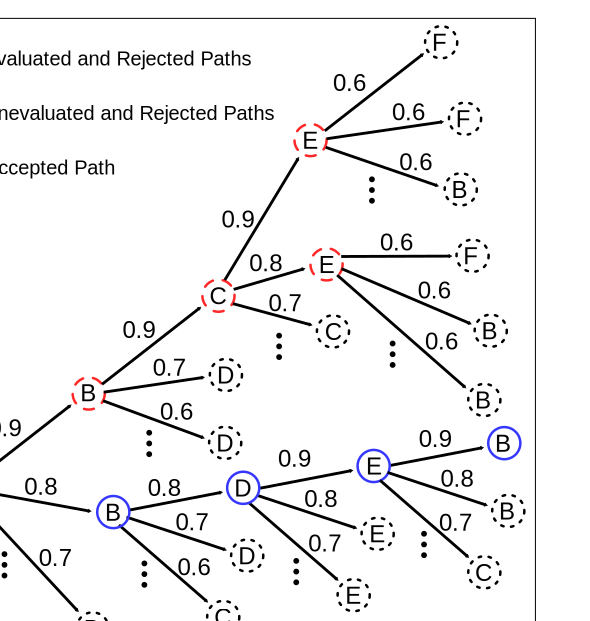
\includegraphics[width=4in]{../issta_profile/profiling/figures/backtracking}
\caption{Example of path prediction through tree search.}
\label{fig:backtracking}
\end{figure}

The branching factor for these trees is large because each node may have thousands of training examples. To simplify the search, we employ the following heuristic. The goal of the heuristic is to find a root-to-leaf path whose edges all have correlation greater than a chosen value $C_{th}$. To evaluate a node, we calculate the correlation of each next edge and sort the nodes in order of decreasing correlation. If the edge with the maximum correlation is greater than $C_{th}$ we continue searching along this edge. Otherwise, we indicate this node as rejected and backtrack along our path so far (\ie toward the root node). As we backtrack we stop at the first node that has an edge to an unevaluated node with correlation greater than $C_{th}$ and search forward along this edge.  In Figure~\ref{fig:backtracking}, $C_{th} = 0.75$, and the search algorithm follows the red dashed nodes from A to B to C to E along the top-most edges. No edge from this E node exceeds $C_{th}$, so the algorithm backtracks to C and then continues forward to the E node with $C_{th} = 0.8$. Again, no edge from here exceeds $C_{th}$, so the algorithm backtracks along C to B to A and moves forward along the accepted blue path.
%4)Reviewer1:What if the path beyond the next marker differs for
%training and profiling signals?  
Because \zop\ identifies paths by matching short subpaths between marker pairs and backtracks when unsuccessful, it can recognize paths that it never observed during training.

This heuristic clearly results in a path where each edge is greater than $C_{th}$, if such a path exists, since \zop\ only follows edges with correlation greater than $C_{th}$. However, it is not guaranteed that all paths that meet our selection criteria correspond to the correct whole program execution path. It is also not guaranteed that a path meeting the selection criteria exists.
%9)Other clarifications for Reviewer1: -We will add references to and
%compare against existing tree-search algorithms. Investigating
%alternative matching algorithms is a possible future research topic.
It is worth noting that many sophisticated heuristic algorithms exist for searching through trees with similar properties~\cite{browne2012,ruml2002,korf1985,biglieri1991}, so we believe that future research in this area can greatly improve the overall path prediction accuracy.
% Our results show this simple algorithm works adequately in practice,
% assuming the refinements mentioned below are implemented.

Two minor refinements are required to make this algorithm practical. First, when correlating the training examples against the profiling waveform it is necessary to correlate the waveforms several times with slight misalignments between the training waveforms and the profiling waveforms and use the best result of all the alignments. This is because the current position in the program is always an estimate, so by trying several different alignments and selecting the best alignment, \zop\ can keep track of the current program location with better accuracy. The second refinement is that the training waveforms for each edge are extended beyond the time position of the next marker so that all the training waveforms starting at a given marker have the same length. This is done by finding the training example for each marker with the longest duration and extending the other training example waveforms for this marker to the same length. This is required to allow fair comparisons between training examples which would otherwise have different lengths (shorter signals are more likely to be more highly correlated due to random chance than longer signals). This approach has the added benefit that (with some preprocessing) all the training waveforms for a given starting marker can be correlated (with several different alignments) against a profiling waveform using a single matrix multiplication which greatly reduces runtime.

%SPACE\subsubsection{Eliminating Redundant or Impossible Search Paths}
\subsubsection{Pruning Search Paths}
Removing nodes before they are evaluated can greatly decrease runtime because the evaluation of each node in this tree is expensive and the tree branches quickly. Some nodes can be rejected quickly without sacrificing much accuracy. For example, suppose two edges W and Z start at a node B and represent BD training waveforms with nearly identical durations. This repetition is common because executions of the same subpath often have roughly the same runtime. Suppose W has higher correlation to the profiling waveform than Z. We can immediately reject Z without evaluating it because the D node following W and the D node following Z occur at the same time in the profiling waveform (since W and Z start at the same time and have the same duration). If W is evaluated and rejected, evaluating Z would just re-evaluate an identical D node with nearly the same start time.

We can eliminate more edges by observing that many marker sequences do not correspond to valid execution paths. To see this, recall that the path prediction execution paths are interprocedural and that we allow an edge from any marker X to a marker Y if an X to Y transition is possible in the profiling program. Then consider a function which contains a single marker F. This function is called from two points A and B in the program, returning at points C and D respectively. Then the only valid marker sequences for this function call would be AFC and BFD. The algorithm described so far would however also evaluate the impossible paths AFD and BFC. Ideally, a fully constrained grammar of all possible paths would be generated to limit the search to possible marker sequences. This grammar could enumerate the set of valid next markers from any node in the search tree. This grammar would be difficult to generate, so instead we keep a function call stack for the currently evaluated execution path and any next marker which would be inconsistent with the call stack is rejected. Note this is a very weak constraint and only eliminates the impossible AFC and BFD sequences when A and B are in different functions.

% there are many more topics that can be described here:
% marker at start and end of function, placement of markers not needed for
%\rob{Rob needs to add description of marker placement, standard library calls, alignment of segments, fixed correlation length, variability of a given path, time between markers varies}

\subsection{Profiling Information}
\label{sec:predict_path}

In the final step of \zop, we construct the paths for the profiling inputs from a set of predicted markers provided by the previous steps. Every consecutive pair of predicted markers represents a set of basic blocks that are executed between two markers by a training input. First, for every training input and every two consecutive pair of markers we extract the basic blocks that are executed between them.  Once \zop\ collects the basic blocks between each pair of markers, it uses this information to generate the predicted whole program basic block path from the sequence of predicted markers. The profiled acyclic paths can be easily identified and counted from this whole program path.

\subsection{Usage Scenarios}

Describing the usage scenarios where \zop\ presents an attractive alternative to existing solutions, we must first be more specific about the requirements for using \zop. First, and most obviously \zop\ requires hardware for demodulation, waveform recording, and signal processing. It is expected these requirements can be met by existing software defined radio receivers. Second, \zop\ also inherits most of the requirements of existing profilers such as instrumentation insertion. Third, \zop\ requires a set of inputs to be used for training. These training inputs must have a coverage of the short subpaths in the program most similar to branch coverage. In most scenarios where an application is to be extensive profiled such a set of inputs exists. The next and final requirement is more subtle. During training the program is instrumented and run to record waveforms and timing information. This raises the question ``If it is possible to run the program with instrumentation, why go through all the trouble of recording and processing waveforms just to count the executed paths?''

There are several reasons for this. First, in many applications it may be feasible to run a program with several short inputs that provide good branch coverage in a testing environment but may not be feasible to instrument the system in a production environment or in the field. This is likely the case for code with realtime requirements or operating system code. In other cases it may be possible to record the profiling information but there may be no easy way to get the profiling information off the device. Second, \zop\ is unique in that it can provide profiling information with no hardware support or direct interaction with the system while it is being profiled. Some computing systems have hardware support for profiling (performance counters, instruction traces, etc.) but these methods require hardware support (both logic on-chip and in some cases large connectors on the PCB) and do affect some system properties such as power consumption. Third, we believe the approach used by \zop\ will find applications beyond profiling such as malware detection and debugging where functioning without instrumentation is desirable for other reasons.
